\section{X-bar Theory}
{\tiny bars represent projection levels}\\
{\tiny introducing 2 bar-levels (e.g. NP and N-bar) allows us to apply recursiveness where necessary, but also avoid it where it would lead to ungrammatical structures}\\
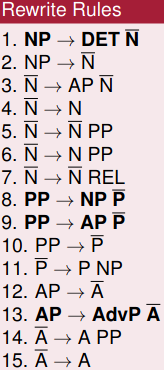
\includegraphics[scale=0.3]{xbar-rules.png}
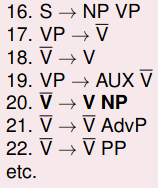
\includegraphics[scale=0.3]{xbar-rules2.png}\\
\scriptsize{X' rules} {\tiny the structural similarities be captured by use X as a placeholder, e.g. \\
X''->specifier'' X'\\
X'->adjunct''X', or X'->X' adjunct''\\
X'->X complement''}\\
\scriptsize{minimal and maximal X' phrases}\\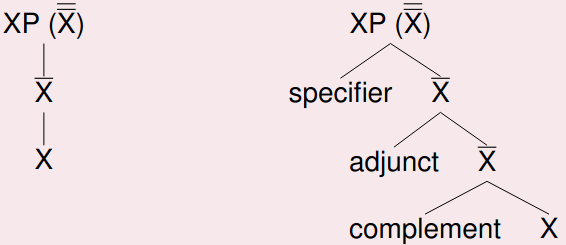
\includegraphics[scale=0.2]{xbar-min-max.png}\\
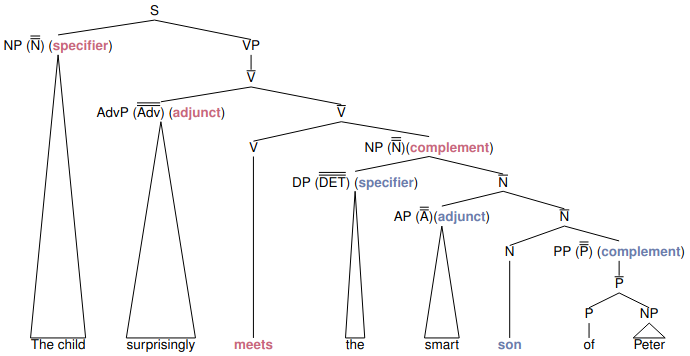
\includegraphics[scale=0.2]{xbar-max.png}\\
\scriptsize{Pros} 
{\tiny explicitely models the productiveness of natural language by recursively applying rules (but also possible in classical PSGs)\\
Abstracts away from particular phrase types and formulates more general rules (X-bar rules)\\
morphological features can be implemented}\\
\scriptsize{Cons} 
{\tiny an inflation of unary branches, analyses of simple sentences daunting\\
Justifying the higher level X rules based on empirical data (i.e. grammatical and ungrammatical sentences) becomes increasingly difficult and controversial.}